\begin{frame}{Representação Intermediária de Código}
    \begin{itemize}
        \item A estrutura de dados gerada pelo compilador, que representa o programa fonte, é chamada de Representação Intermediária (do inglês, \textit{intermediate representation}, ou IR) \cite{cooper2014}.

    \end{itemize}
\end{frame}

\begin{frame}{Representação Intermediária de Código}
    \begin{itemize}
        \item Um compilador pode utilizar uma ou mais IRs, podendo variar desde uma estrutura em árvore ou grafo até alguma outra linguagem de programação, como C e representações de código funcional \cite{aho2008compilers}.

        \item []

        \item[] \begin{figure}
            \centering
            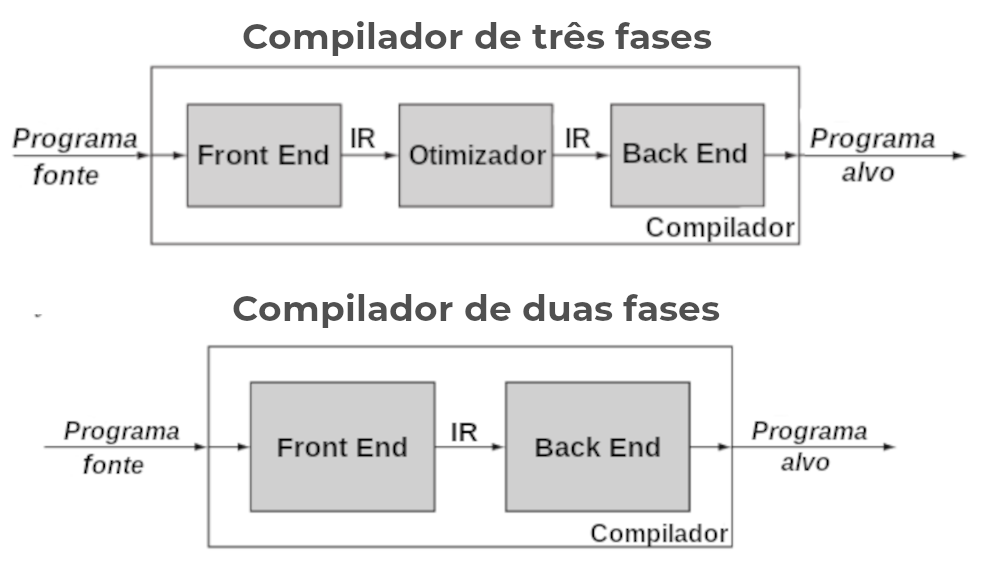
\includegraphics[width=.56\textwidth]{Figuras/compilador.png}
            \caption{Tipos de Compilador \cite{cooper2014}}
            \label{fig:comp}
        \end{figure} 
    \end{itemize}
\end{frame}